\documentclass[fleqn,10pt]{physiome}
% Use option lineno for line numbers 

%for links
%\usepackage{hyperref}

\newcommand{\ca}{Ca$^{2+}$}
\newcommand{\cas}{Ca$^{2+}$ }
\newcommand{\cacyt}{[Ca$^{2+}$]$_i$}
\newcommand{\cacyts}{[Ca$^{2+}$]$_i$ }
\newcommand{\ipr}{IP$_3$R }
\newcommand{\ip}{IP$_3$ }
\newcommand{\nas}{Na$^+$ }
\newcommand{\na}{Na$^+$}
\newcommand{\cl}{Cl$^-$ }
\newcommand{\po}{K$^+$ }
\newcommand{\pos}{K$^+$  }


\articletype{Original}
%% Choose from Original, Retrospective, Review, Letter

\title{Steady-state Approximations for Hodgkin-Huxley Cell Models: Towards Multi-scale Models of Uterine Smooth Muscle}

\author[1][s.means@auckland.ac.nz]{Shawn A. Means}
\author[1]{Alys R. Clark}
\author[1]{Leo K. Cheng}
\affil[1]{Auckland Bioengineering Institute, University of Auckland, New Zealand}
%\affil[2]{Address of second author}

%% The following lines can be omitted when submitting;
%% information will be added by editors
\publicationdate{30 Oct 2023}
\editor{David P. Nickerson}
\curator{Shelley Fong}
\submitteddate{15 Dec 2022}
\accepteddate{18 Sep 2023}
\citethisas{Means et al. (2023)\\Steady-state Approximations for Hodgkin-Huxley Cell Models: Towards Multi-scale Models of Uterine Smooth Muscle. Physiome.}{10.36903/physiome.24439204}
\begin{document}

\maketitle

\begin{abstract}
The \cite{tong2011} publication presents a comprehensive mathematical model of electro-mechanical behaviour in a uterine smooth muscle cell. It incorporates ion channel currents into a classic Hodgkin-Huxley membrane voltage formulation as well as \cas concentration dynamics with pumps and exchangers. Mechanical force generation by way of the Hai-Murphy smooth muscle cell model is computed based on the \cas concentrations. The `full' Tong 2011 model (FTM) includes nineteen ordinary differential equations for the ion channel activation/inactivation variables out of a total of 105 equations overall. An effort at reducing the FTM into a smaller number of equations for computational efficiency -- the `reduced' Tong model (RTM) -- aims at reproducing the overall behaviour of the FTM without excessive detail. We present here the CellML implementation of the RTM for simulating the FTM within the context of the reduced model's primary publication as derived from the \cite{tong2011} model.
\end{abstract}

\keywords{uterine smooth muscle, computational model, reduction order, cellular calcium, myometrial contraction, CellML}

\primarypubs[10.36903/physiome.24439204]{reduced_usmc}{means2022}
%\primarypubs[10.1037a0000000]{sample}{Aivazian917,Bloss029983}

\section{Introduction}
Balancing computational tractability and realism is a persistent concern for mathematical modeling. Of the published uterine smooth muscle cell (USMC) models, the \cite{tong2011} version is somewhat of a gold standard for the cell type, yet encompasses a substantial computational expense in solving the nineteen ODEs amongst the full suite of 105 equations for the `full' Tong Model (FTM). We present the mathematical model for a `reduced' Tong Model (RTM) aimed at reproducing the overall behaviour of the FTM but with reduced computational expense as developed by \cite{means2022}. Both the FTM and RTM are available in the Physiome Model Repository (PMR) \citep{pmr2011}, and we utilise the implementations provided for presenting the results given in the RTM model primary publication of \cite{means2022} comparing the FTM and RTM simulations.




%\begin{figure}[ht]\centering
%\includegraphics[width=0.5\linewidth]{./pics/usmc_comp_burs_fig6_tong_fig12_v1p1}
%\caption{Caption}
%\label{fig:tong_bursztyn_comp1}
%\end{figure}


\section{Model description}

\subsection{Primary Publication}

The FTM model \citep{tong2011} assembles numerous ion channel submodels for representing the membrane voltage ($V_m$) with a Hodgkin-Huxley formalism. Of these submodels, the FTM includes one \na, two \cas ($V_m$-gated), five \pos as well as a non-specific Cation channel and a `hyperpolarisation' \nas and \pos channel. These entail a total of nineteen ODEs for activation and inactivation variables. Additional \cas dynamic mechanisms such as a plasma-membrane ATP-ase pump and the \na-\cas exchanger are included and another exchanger, the \na-\pos transporter appears as well. \cacyts in turn provides activation of a Hai-Murphy cross-bridge model describing contraction for smooth muscles \cite{haimurphy1988}. For the RTM, only the ion channel mechanisms and transporters are considered for reduction; particularly, the activation and inactivation variables are considered in turn for steady-state approximations. The primary paper of \cite{means2022} is then the focus of the model consideration: comparison between presented results in Means, et al. of the RTM with the FTM is provided in this article demonstrating CellML implementations of both the reduced and full model variants.

\subsection{CellML Models}

%Implementations of both the FTM and RTM are available in the Physiome Model Repository (PMR) at \href{https://models.physiomeproject.org/workspace/261}{here} and \href{https://models.physiomeproject.org/workspace/8bc}{here} https://models.physiomeproject.org/workspace/261 and https://models.physiomeproject.org/workspace/8bc, respectively. This article focuses on the reproduction of results presented in the primary article of Means, et al. \cite{means2022} and not results presented in Tong, et al. \cite{tong2011}, and is thus arranged accordingly. 

Implementations of both the FTM and RTM are available in the Physiome Model Repository (PMR) \href{https://models.physiomeproject.org/workspace/261}{here} and \href{https://models.physiomeproject.org/workspace/8bc}{here}, respectively. This article focuses on the reproduction of results presented in the primary article of \cite{means2022} and not results presented in \cite{tong2011}, and is thus arranged accordingly. 

Individual results of the primary article are then organised according to reproduction of key results from the FTM associated article. Variations of parameters and enabling or disabling of full dynamical variables or utilisation of their steady-state approximating equivalents are noted where suitable. 

Two sets of simulations experiments are presented in the results of primary article:

\begin{enumerate}
	\item Reproduction of experimental data simulated in Fig. 12 of FTM using the RTM-described `Standard Simulation Protocol':
	\begin{enumerate}
		\item Applied stimulus, $I_{app}$, of -0.5 pA/pF, duration 2 seconds.
		\item $V_m$, \cacyts and force generation output comparison.
	\end{enumerate}
	\item Reproduction of experimental data simulated in Fig. 11 of FTM:
	\begin{enumerate}
		\item Applied stimulus, $I_{app}$, of -0.9 pA/pF, duration 9 seconds.
		\item Applied stimulus, $I_{app}$, of -0.4 pA/pF, duration 9 seconds.
		\item Depolarising \pos elevated external concentration.
		\item Applied stimulus, $I_{app}$, of -0.3 pA/pF, duration 9 seconds.
		\item Applied stimulus, $I_{app}$, of -0.2 pA/pF, duration 49 seconds.
		\item $V_m$ output comparison.
	\end{enumerate}
\end{enumerate}

%Details of parameter variations and ion channel variable computations are provided as noted below as well as referred to in the primary publication. 

Details of parameter variations are noted in the corresponding figure subtitles as well as referred to in the primary publication. 

\section{Model Results}

Note, the originating simulation data was generated in OpenCOR, as well as the reproduction for both the FTM and RTM using PMR implementations of the respective CellML models; no extraction of figures was performed for this presentation. All figures generated with CellML implementation with minor variations in applied stimulus strength or duration ($I_{stim}$) conductances (i.e., $g_{K1}$) as noted throughout and readily reproducible given said variations when performed manually in the CellML file available at the PMR. 

\subsection{Standard Simulation Protocol (SSP)}

The SSP formed the basis for a test case of accuracy and performance with the RTM versus the FTM, given above noted parameters of stimulus and duration. All initial conditions of the numerous concentrations, membrane voltage and activation or inactivation variables are as noted in the FTM (and RTM) description. For the FTM, the result is itself a reproduction of experimental traces given in Okabe, et al. \citep{okabe1999}; the result shown  in Fig. \ref{fig:ssp} is generated with the Tong, 2011 PMR CellML implementation. The RTM generates the observed reproduction of results as shown utilising the Reduced Tong, 2011 PMR CellML implementation deploying steady-state approximations of the full model's ordinary differential equations. Both the FTM and RTM curves are as demonstrated from the originating publication, where the FTM result is shown with black '+' and RTM with a blue trace. Differences between them are a result of the reduction method described in the primary publication, Means, et al. \citep{means2022}. Note, all initial conditions and parameter values are set to defaults in the provided CellML implementations at the PMR.


\begin{figure}[ht]\centering
\begin{tabular}{c c}
\centering
(a) & 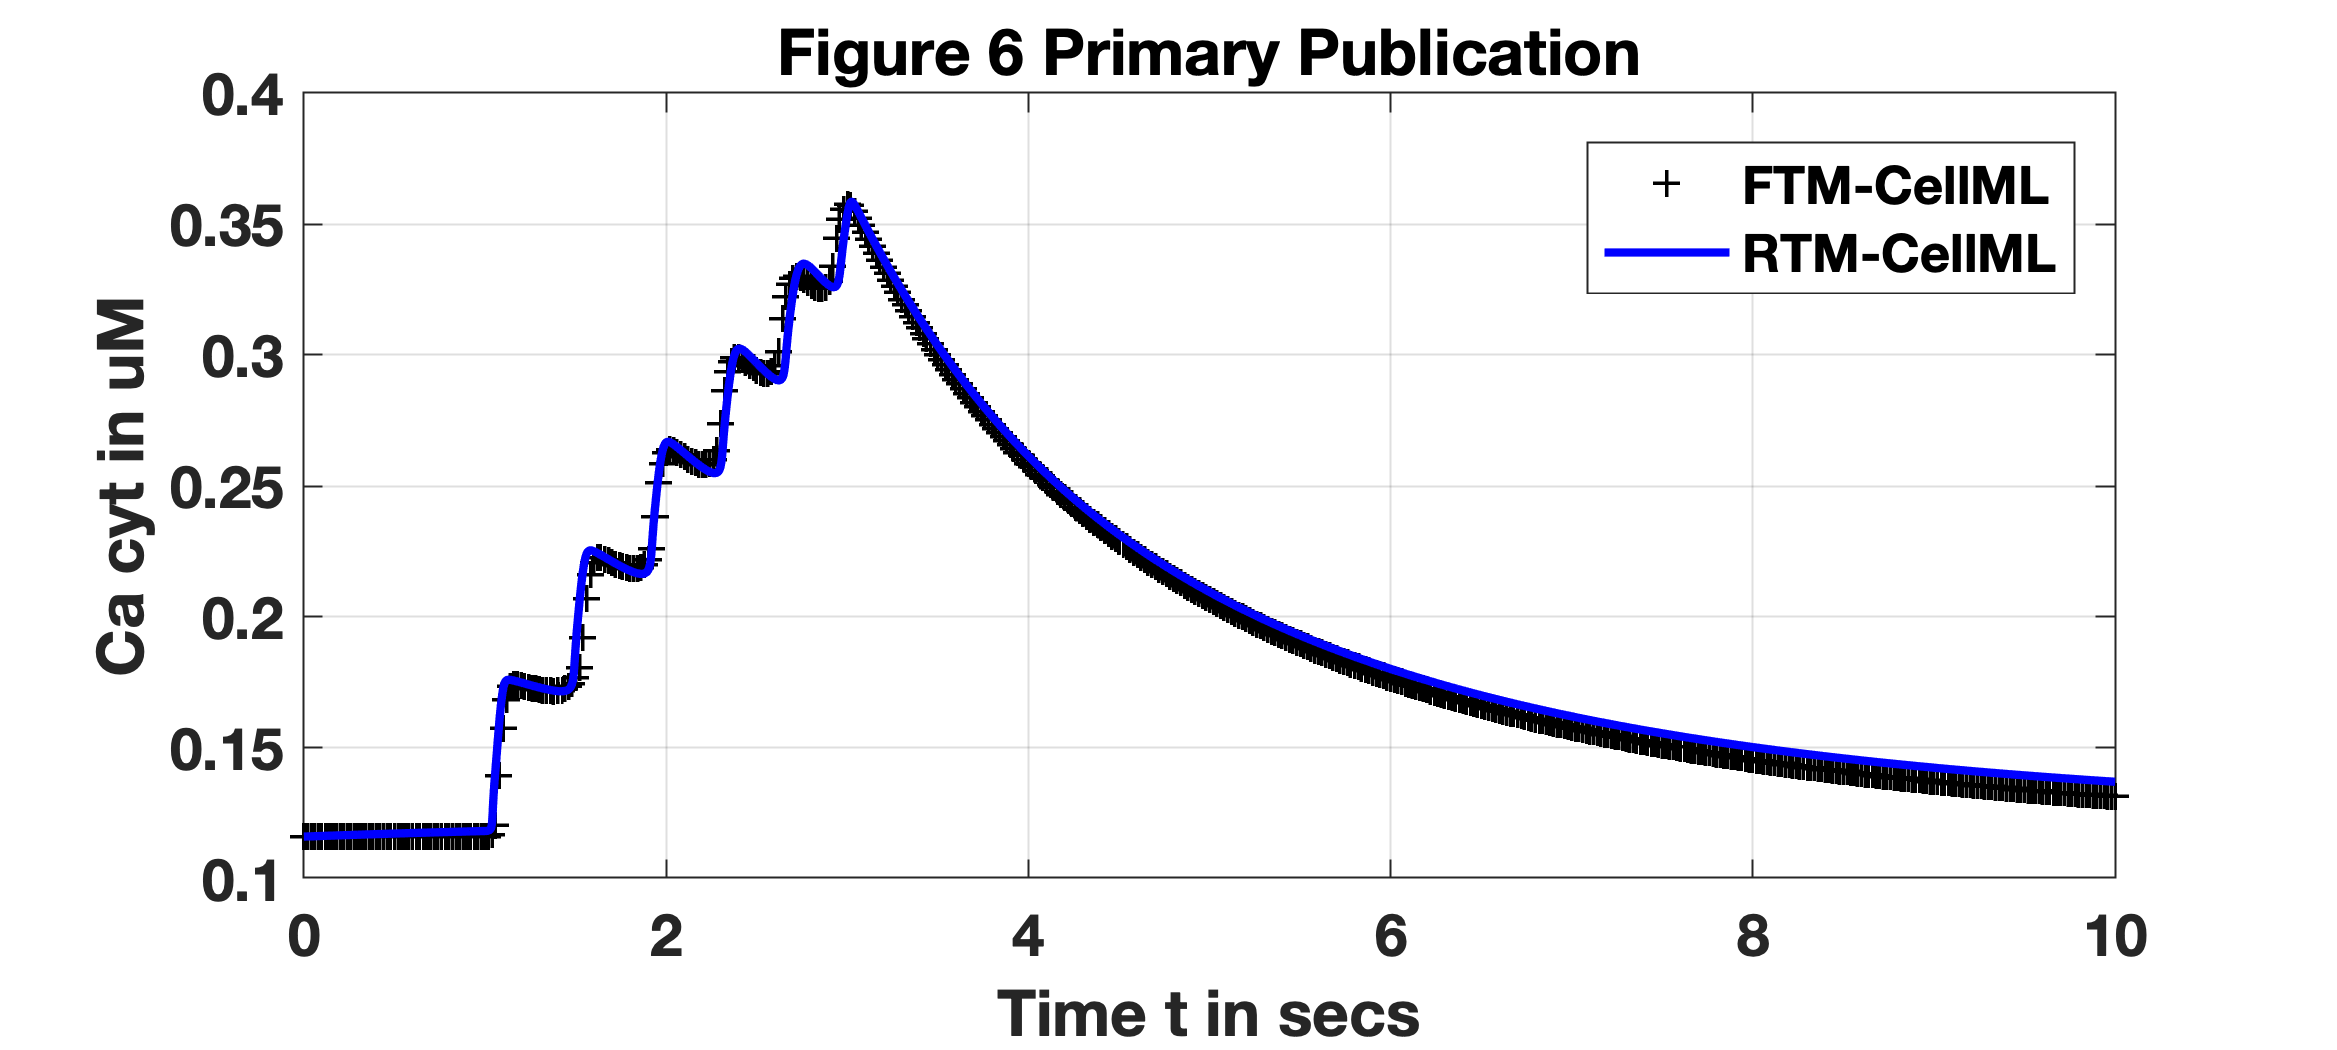
\includegraphics[scale=0.35]{./pics/fig6_cacyt}  \\
(b) & 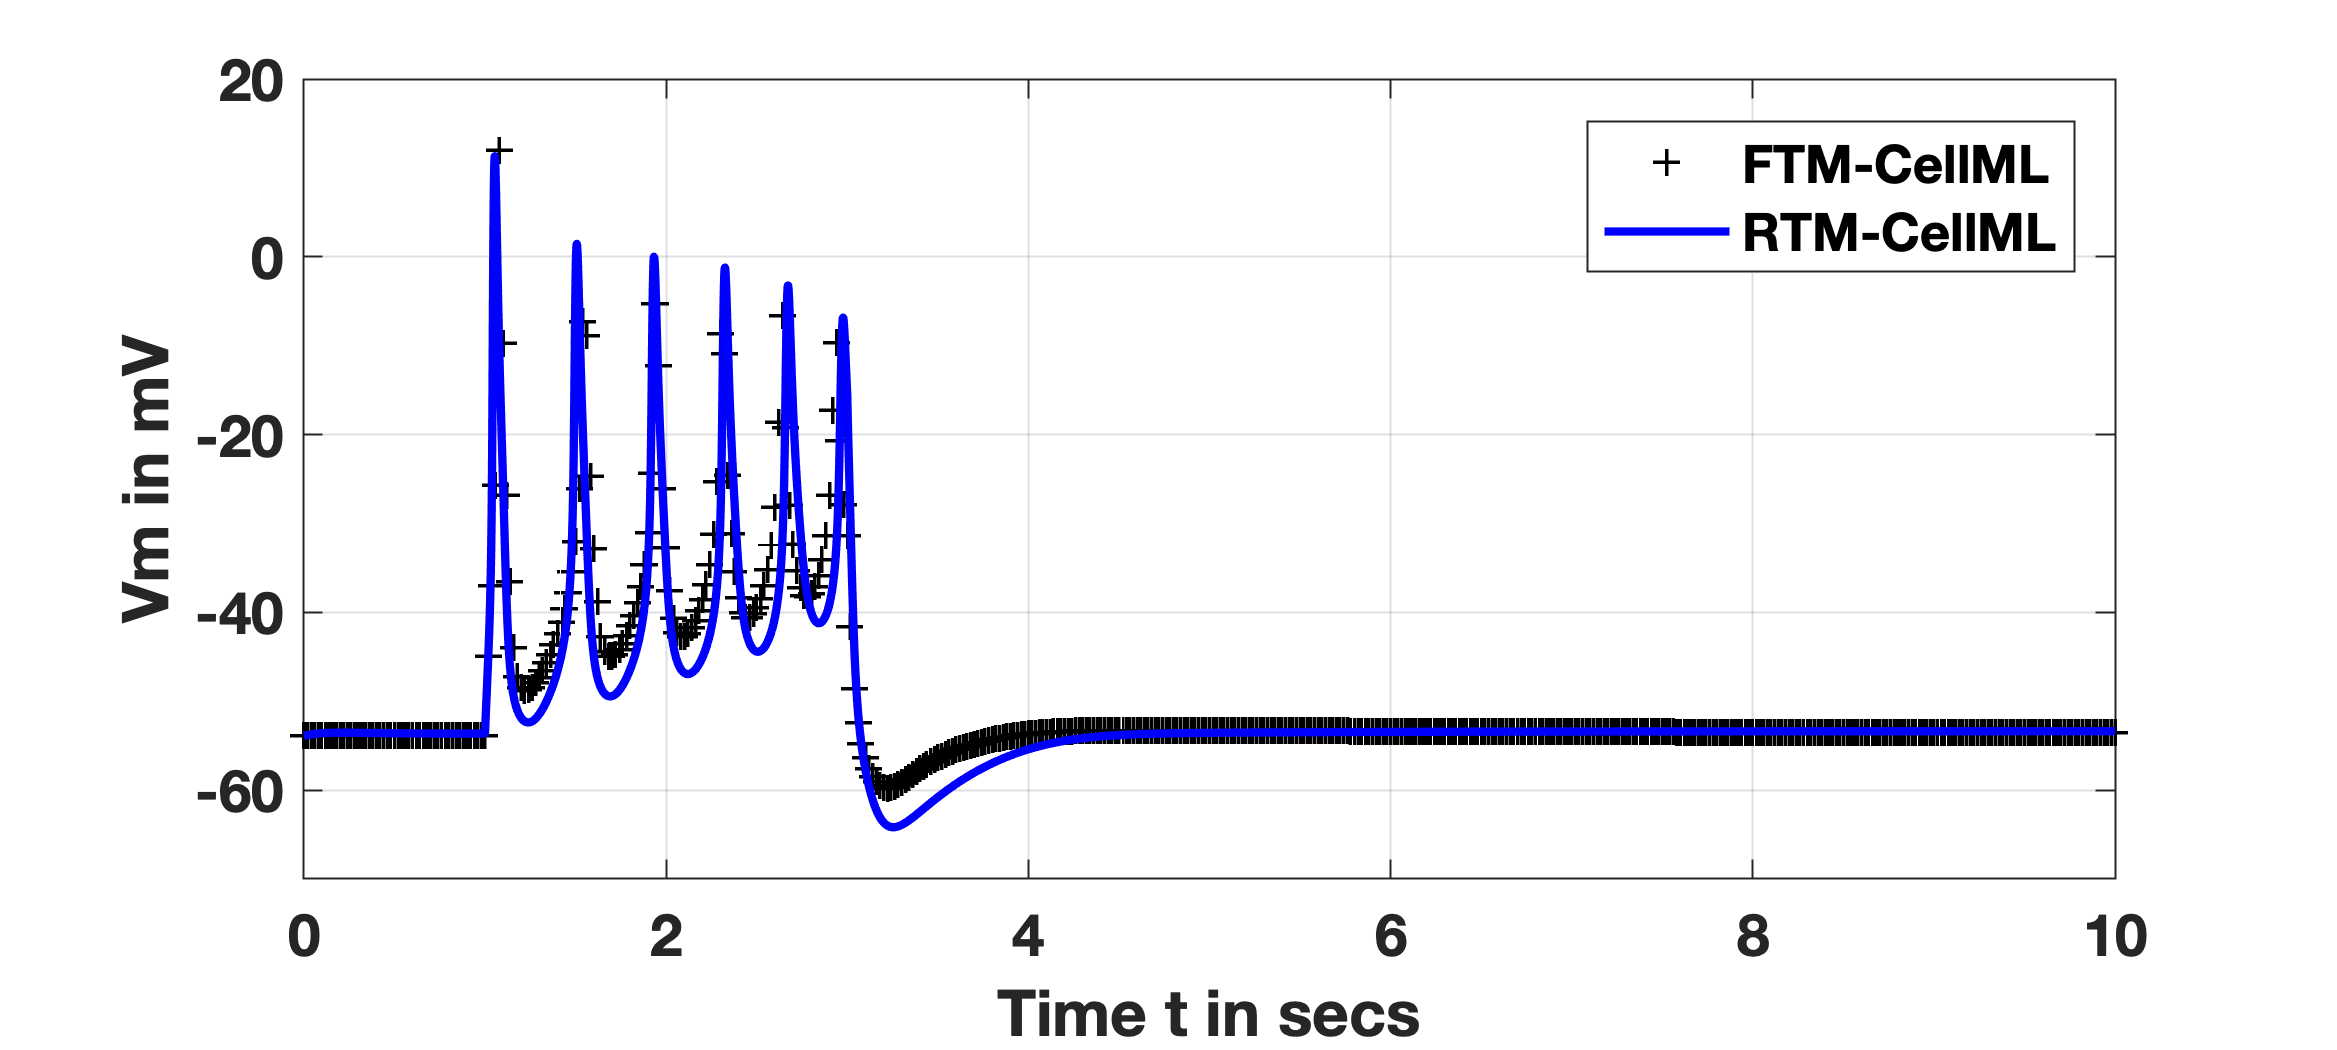
\includegraphics[scale=0.35]{./pics/fig6_vm}  \\
(c) & 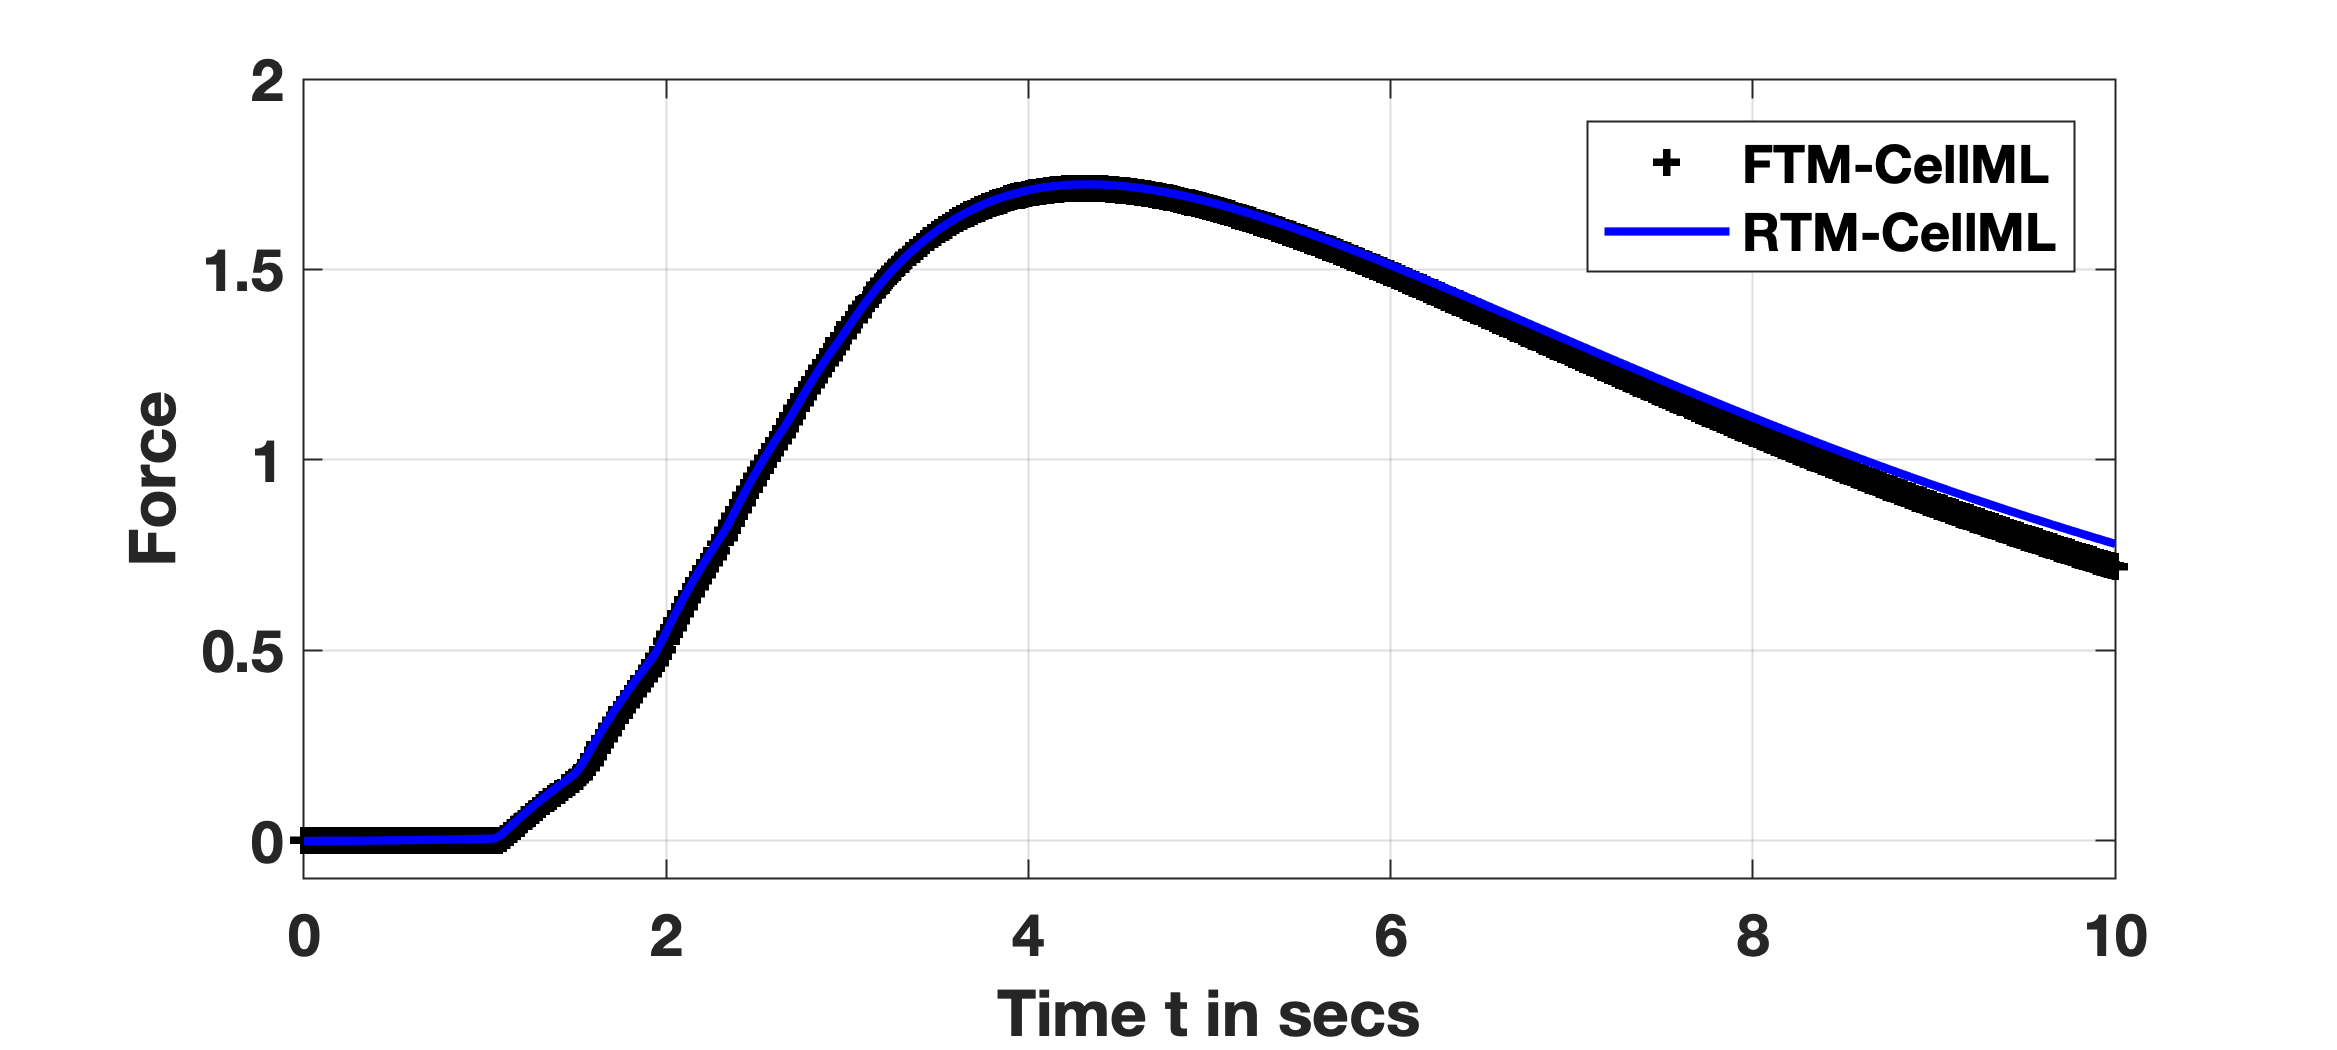
\includegraphics[scale=0.35]{./pics/fig6_force}  \\
\end{tabular}
\caption{SSP Reproduction: FTM and RTM results: black '+' and blue trace, respectively. All initial conditions are identical between them with an applied stimulus, $I_{stim}$ of -0.5 pA/pF for two seconds initiated at time $t=1.0$ secs.}
\label{fig:ssp}
\end{figure}

\subsection{$I_{app}$ Variations}

The primary paper demonstrates functionality of the RTM model as a whole applied to scenarios demonstrated in Figure 11 of the original Tong, et al. paper where applied stimulus, $I_{app}$ is varied along with a test depolarising pulse of extracellular potassium, $K^+_o$. Plots show in this instance data taken from the originating OpenCOR computations for the primary paper (labeled 'Means, et al.') and regenerating code ('CellML') with black '+' and blue traces, respectively (Figure \ref{fig:variation}). 'Base case' for RTM results generated include variations to channel conductances as described in the primary publication; variants thereof described as such as noted primarily include changes to $I_{stim}$ or $g_{K1}$ (see Fig. \ref{fig:variation}). Deviations in results between the original data traces and reproduction are minimal if at all - particularly with the longer-term stimulus of Panel (e). Each result stems from gradual reduction in $I_{app}$ with the suite of varied conductances for the channels included in the RTM along with steady-state approximations; note, there is no comparison trace here with the FTM result of Figure 11, Tong, et al. 2011 \citep{tong2011}. Nevertheless, the primary paper results given in Figure 7 of Means, et al. \citep{means2022} demonstrate production of each trace with the appropriate value of $I_{stim}$ as noted: -0.9, -0.4, -0.3 and -0.2 pA/pF for Panels (a-b) and (d-e). The longer-time duration for these results of 9 seconds and longer with (e) generate the longer set of action potentials as well. Note, Panel (e) includes a variation to the conductance of the $K1$ potassium channel with $g_{K1}$ = 0.75 pA/pF. Alternatively, Panel (c) of Fig. \ref{fig:variation} shows not a variation of $I_{stim}$ but rather effect of a depolarising $K^+_o$ pulse, where concentration of extracellular \po is set to 10 mM. These variations are applied manually to the provided RTM CellML implementation available at the PMR; no automated scripts generate these results as of writing this article. 

Traces shown in Fig. \ref{fig:variation}  reproduce results given in Means, et al. aimed at showing ability of RTM to mimic production of the experimental traces of Wilde and Marshall, 1988 \citep{wilde1988} and Meisheri, 1979 \citep{meisheri1979}, as referenced in Tong, et al. The OpenCOR implementations of both the FTM and RTM variants of Tong, et al. 2011 demonstrate ability to produce results from both Tong, et al., 2011 and Means, et al.


\begin{figure}[ht]\centering
%\begin{tabular}{c c c c}
\centering
%(a) & \includegraphics[scale=0.35]{../pics/fig7a_istim_-0p9_vm_fix_wcomp2} & (d) & \includegraphics[scale=0.35]{../pics/fig7c_istim_-0p3_vm_fix_wcomp2} \\
%(b) & \includegraphics[scale=0.35]{../pics/fig7b_istim_-0p4_vm_fix_wcomp2} & (e) & \includegraphics[scale=0.35]{../pics/fig7d_istim-0p2_tdur50_gk1_0p75_vm_fix_wcomp2}\\
%(c) & \includegraphics[scale=0.35]{../pics/fig7b_ko_10mM_vm_fix_wcomp2}  \\
%\includegraphics[scale=0.35]{../pics/fig7a_istim_-0p9_vm_fix_wcomp2} & (a)  & \includegraphics[scale=0.35]{../pics/fig7c_istim_-0p3_vm_fix_wcomp2} & (d) \\
%\includegraphics[scale=0.35]{../pics/fig7b_istim_-0p4_vm_fix_wcomp2} & (b) & \includegraphics[scale=0.35]{../pics/fig7d_istim-0p2_tdur50_gk1_0p75_vm_fix_wcomp2} &  (e) \\
%\includegraphics[scale=0.35]{../pics/fig7b_ko_10mM_vm_fix_wcomp2} & (c) \\
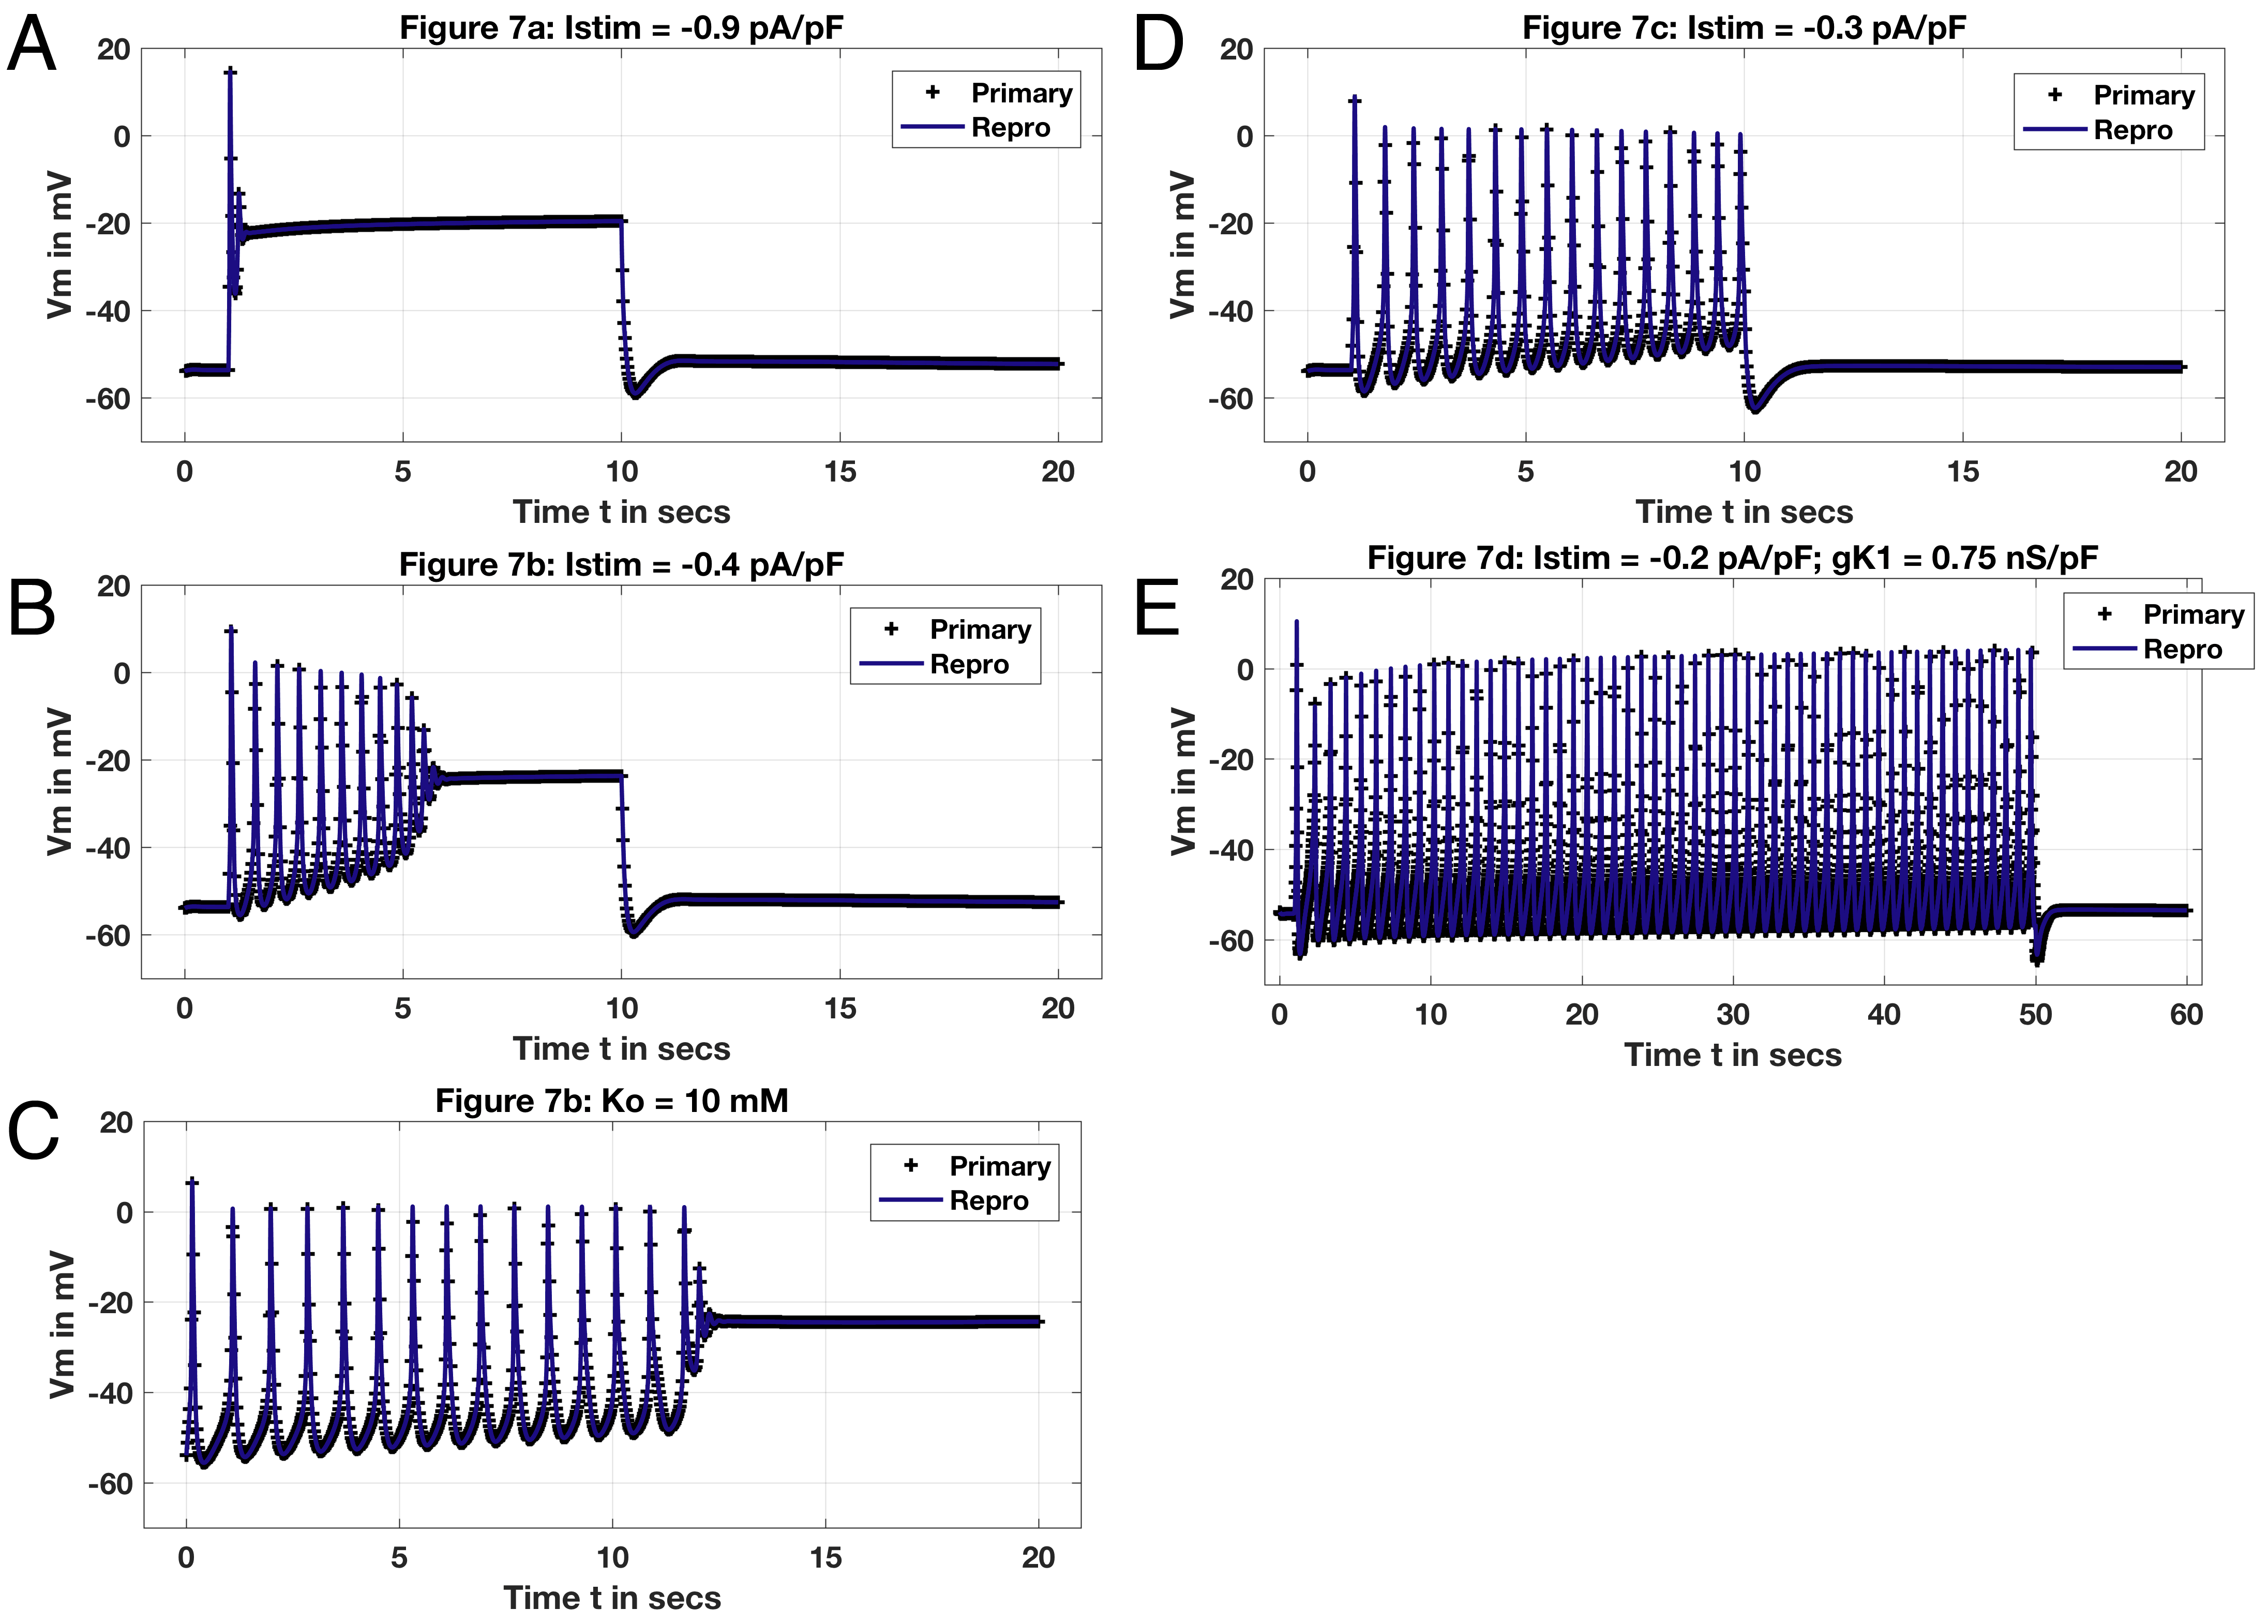
\includegraphics[scale=0.35]{./pics/sig2_assby-01}
%\end{tabular}
\caption{Reproduction of $I_{stim}$ variants. Panel (a): I$_{stim}$=-0.9 pA/pF, duration 9 seconds ($t_0$ = 1 to $t_f$ = 10 secs; all parameters identical to base case). Panel (b): I$_{stim}$=-0.4 pA/pF, duration 9 seconds  ($t_0$ = 1 to $t_f$ = 10 secs; all parameters identical to base case). Panel (c) $I_{stim}$=0; external $K^+_o$ pulse 10 mM (all parameters otherwise identical to base case). Panel (d):  I$_{stim}$=-0.3 pA/pF, duration 9 seconds (all parameters identical to base case).  Panel (e) I$_{stim}$=-0.2 pA/pF, duration 49 seconds, $g_{K1}$=0.75 pA/pF (all parameters otherwise identical to base case).}
\label{fig:variation}
\end{figure}

\section{Discussion}

We demonstrated reproducibility of the RTM version of the FTM as shown in the primary article of Means, et al. \citep{means2022}. We utilised the available CellML implementation of the RTM available at the PMR for said demonstration, as well as the FTM implementation for comparisons where noted. Each result shown is a replication of the original results given in Means, et al. with only a minor variation in $g_{K1}$as noted in for the $I_{stim}$ variants presented in Fig. \ref{fig:variation} Panel (e). All results shown here are readily computable by way of the CellML models in the repository with slight modifications to the parameter values and stimulus protocols as detailed above. 

\section{Acknowledgement}
 
This work was funded, in part, by grants from the New Zealand Ministry of Business Innovation and Employment's Ministry of Business, Innovation and Employment's Catalyst: Strategic Fund.

%\subsection{Primary Publication}
%
%Every \emph{Physiome} article needs to be associated with one or more Primary Publications. The Primary Publication is an experimental/modelling paper describing the model(s), that has been accepted to a peer-reviewed journal in the field of physiological modelling. The Primary Publication shows that the model is validated by describing the experiments and data, and the model(s) fit to the data, as well as the biological background and why the model is important.
%\emph{Physiome} articles focus on reproducibility and reuse, but do not deal with the validation or scientific relevance of the models.
%
%You can list the primary publications in a .bib file, then insert them after the \verb|\keywords{...}| using the \verb|\primepubs| command:
%
%\verb|\primepubs{name of .bib file}{BibTeX keys of the publications}|
%
%If your code is online, provide the link as an optional argument to \verb|\primepubs|:
%
%\begin{verbatim}
%    \primepubs[link to the model code]
%      {name of .bib file}{BibTeX keys of the publications}|
%\end{verbatim}
%
%If you are authoring and compiling this template on your own machine, you will need to run an extra step \verb|bibtex primepub| to generate them in the final PDF. If you wish, you can use \texttt{latexmk}, \texttt{arara} or \texttt{Make} to automate this step.

%\subsection{Some \LaTeX{} Examples}
%\label{sec:examples}
%
%Use section and subsection commands to organize your document. \LaTeX{} handles all the formatting and numbering automatically. Use \verb|\autoref| and \verb|\label| commands for cross-references, e.g.~\autoref{sec:examples}, \autoref{eq:sum}, \autoref{fig:view}, \autoref{tab:widgets}. You can still use the more common \verb|\ref|, but this will only generate the (sub)section/table/figure/equation number: \ref{tab:withnotes}. 
%
%\subsection{Figures and Tables}
%
%Use the table and tabular commands for basic tables --- see \autoref{tab:widgets}, for example. \autoref{tab:withnotes} shows a larger example with \emph{table notes}. You can upload a figure (JPEG, PNG or PDF) using the project menu. To include it in your document, use the \verb|\includegraphics| command as in the code for \autoref{fig:view} below. Captions are always justified and start from the left; don't try to change the alignment.
%
%If you prefer, you can place all your image files in a folder. Remember to include the folder path in your \verb|\includegraphics| command, or use `\verb|\graphicspath|` to specify the path to the folder in which all your image files can be found.
%
%\begin{figure}[ht]\centering
%\includegraphics[width=0.5\linewidth]{frog}
%\caption{An example image of a frog.}
%\label{fig:view}
%\end{figure}
%
%\begin{table}[ht]\centering
%\caption{An example table.}\label{tab:widgets}
%\begin{tabular}{l r}
%\toprule
%Item & Quantity \\\midrule
%Candles & 4 \\
%Fork handles & ?\\
%\bottomrule
%\end{tabular}
%\end{table}
%
%\begin{table}[hbt!]\centering
%\begin{threeparttable}
%\caption{An example table with tablenotes}\label{tab:withnotes}
%
%\begin{tabular}{lccrr}
%\toprule
%Variables & JKL ($n=30$) & Control ($n=40$) & MN & $t$ (68)\\
%\midrule
%Age at testing & 38 & 58\tnote{1} & 504.48 & 58 ms\\
%Age at testing & 38 & 58 & 504.48 & 58 ms\\
%Age at testing & 38 & 58 & 504.48 & 58 ms\\
%Age at testing & 38 & 58 & 504.48 & 58 ms\\
%Age at testing\tnote{2} & 38 & 58 & 504.48 & 58 ms\\
%Age at testing & 38 & 58 & 504.48 & 58 ms\\
%\bottomrule
%\end{tabular}
%\begin{tablenotes}
%\item[1] JKL, just keep laughing.
%\item[2] MN, merry noise.
%\end{tablenotes}
%\end{threeparttable}
%\end{table}
%
%\subsection{Citations}
%
%LaTeX formats citations and references automatically using the bibliography records in your .bib file, which you can edit via the project menu. Use the \verb|\citet| command for a text citation, like \citet{lees2010theoretical}, and the \verb|\citep| command for a citation in parentheses \citep{McQuilton01012012}.
%
%\subsection{Mathematics}
%
%\LaTeX{} is great at typesetting mathematics. Let $X_1, X_2, \ldots, X_n$ be a sequence of independent and identically distributed random variables with $\text{E}[X_i] = \mu$ and $\text{Var}[X_i] = \sigma^2 < \infty$, and let
%\begin{equation}\label{eq:sum}
%S_n = \frac{X_1 + X_2 + \cdots + X_n}{n}
%      = \frac{1}{n}\sum_{i}^{n} X_i
%\end{equation}
%denote their mean. Then as $n$ approaches infinity, the random variables $\sqrt{n}(S_n - \mu)$ converge in distribution to a normal $\mathcal{N}(0, \sigma^2)$.
%
%\subsection{Lists}
%
%You can make lists with automatic numbering \dots
%
%\begin{enumerate}[noitemsep] 
%\item Like this,
%\item and like this.
%\end{enumerate}
%\dots or bullet points \dots
%\begin{itemize}[noitemsep] 
%\item Like this,
%\item and like this.
%\end{itemize}
%\dots or with words and descriptions \dots
%\begin{description}
%\item[Word] Definition
%\item[Concept] Explanation
%\item[Idea] Text
%\end{description}

%\section{Model results}
%
%Efforts at hybridising the Bursztyn and Tong USMC models encounter issues of disparate scaling for behaviour of the L-type Ca$^{2+}$ channel as illustrated in Fig. [REF].
%
%\begin{figure}[ht]\centering
%\includegraphics[width=0.5\linewidth]{./pics/tong_bursztyn_hybrid_Ical_Ina_ik1_comp1}
%\caption{Demonstration of the hybrid Bursztyn-Tong USMC model illustrating difference between the two implementations for the L-type Ca$^{2+}$ channel ($I_{caL}$, panel 2). These differences in current -- although qualitatively similar -- are driven by the underlying and quite different representations of the channel. The Tong formulation (see Eqn. [REF]) with an activation and in-activation variable experiences significantly lower overall activity and current strengths, whereas the Bursztyn by virtue of including only an activation term (see Eqn. [REF]) exhibits far stronger activity (blue-traces).}
%\label{fig:cur_comp_ltype1}
%\end{figure}

% \section{Discussion}

% Quam suscipit ut quidem et animi numquam consectetur et. Nihil et commodi ut officia eveniet beatae qui. Placeat accusantium eius consequatur animi nisi sed. Pariatur et dolores tempore velit similique voluptatem similique error.

% Quam suscipit ut quidem et animi numquam consectetur et. Nihil et commodi ut officia eveniet beatae qui. Placeat accusantium eius consequatur animi nisi sed. Pariatur et dolores tempore velit similique voluptatem similique error.

\bibliography{reduced_usmc}
%\bibliography{sample}

\end{document}